\section{问题分析}

\subsection{问题一分析}
题目要求建立模型描述折叠桌的动态变化图,由于在折叠时用力大小的不同,我们不能描述在某一时刻折叠桌的具体形态,但我们可以用每根木条的角度变化来描述折叠桌的动态变化。首先,我们知道折叠桌前后左右对称,我们可以运用几何知识求出四分之一木条的角度变化。最后,根据初始时刻和最终形态两种状态求出桌腿木条开槽的长度。



\subsection{问题二分析}
题目要求从折叠桌的稳固性好、加工方便、用材最少三个角度,确定设计加工参数。我们可以从应力、支撑面积考虑稳固性,从开槽长度考虑加工方便,从木板长度考虑用材最少。而它们之间又是相互制约,我们需要确定最优设计加工参数,可以建立非线性规划模型,用lingo软件来求解最优设计加工参数(平板尺寸、钢筋位置、开槽长度等),这里以合力的方向(斜向上)与最长木条(桌腿)的夹角方向最小为目标函数,以木条所承受应力小于木条的许用应力、支撑面积大于桌面面积、木条的开槽长度小于木条本身长为约束条件。
\begin{figure}[!h]
\centering
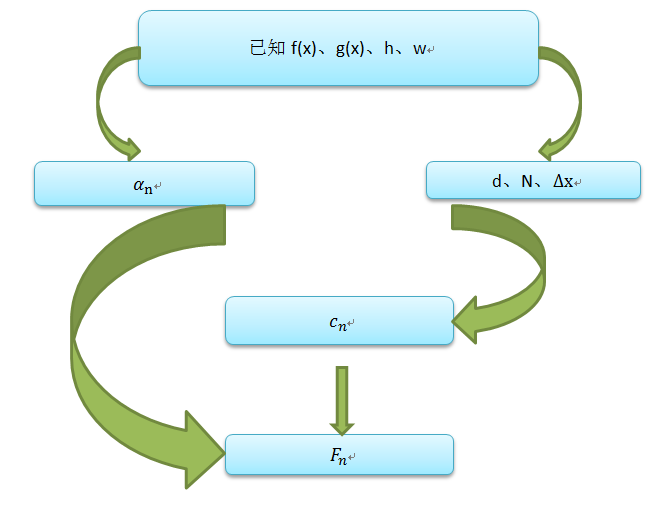
\includegraphics[width=.7\textwidth]{1.png}
\caption{问题三流程图}
\end{figure}
\subsection{问题三分析}
题目要求制作软件的意思就是客户给定折叠桌高度、桌面边缘线的形状大小和桌脚边缘线的大致形状,将这些信息输入程序就得到客户想要的桌子。我们在求解最优设计加工参数时,自行给定桌面边缘线形状(椭圆、相交圆等),桌脚边缘线形状,折叠桌高度,应用第二问的非线性规划模型,用MATLAB软件绘制折叠桌截面图,得到自己设计的创意平板折叠桌。